\documentclass[conference,letterpaper]{IEEEtran}
\IEEEoverridecommandlockouts
\usepackage{cite}
\usepackage{amsmath,amssymb}
\usepackage{graphicx}
\usepackage{booktabs}
\usepackage{array}
\usepackage{xcolor}
\usepackage{url}
\usepackage[hidelinks]{hyperref}

% Every result below is a macro generated by make_numbers.py from the
% evaluation outputs; nothing is typed by hand.
% AUTO-GENERATED by make_numbers.py — do not edit by hand
% source: ../final2
\newcommand{\Pilot}{0}
\newcommand{\PilotNote}{}
\newcommand{\NSubj}{23}
\newcommand{\NRec}{160}
\newcommand{\NSz}{194}
\newcommand{\NHours}{220}
\newcommand{\NColdStart}{15}
\newcommand{\NRecAll}{165}
\newcommand{\NSzAll}{198}
\newcommand{\NHoursAll}{225}
\newcommand{\PyBSens}{5.7\%}
\newcommand{\PyBDet}{11}
\newcommand{\PyBCI}{2--12\%}
\newcommand{\PyBMacro}{10.0\%}
\newcommand{\PyBMacroCI}{3--18\%}
\newcommand{\PyBFAh}{0.32}
\newcommand{\PyBFAday}{8}
\newcommand{\PyBFACI}{0.20--0.48}
\newcommand{\PyBLat}{26.3}
\newcommand{\PyASens}{21.1\%}
\newcommand{\PyADet}{41}
\newcommand{\PyACI}{14--29\%}
\newcommand{\PyAMacro}{25.4\%}
\newcommand{\PyAMacroCI}{15--36\%}
\newcommand{\PyAFAh}{2.82}
\newcommand{\PyAFAday}{68}
\newcommand{\PyAFACI}{2.00--3.86}
\newcommand{\PyALat}{28.4}
\newcommand{\FwBSens}{75.3\%}
\newcommand{\FwBDet}{146}
\newcommand{\FwBCI}{60--94\%}
\newcommand{\FwBMacro}{87.6\%}
\newcommand{\FwBMacroCI}{79--95\%}
\newcommand{\FwBFAh}{18.29}
\newcommand{\FwBFAday}{439}
\newcommand{\FwBFACI}{15.19--21.21}
\newcommand{\FwBLat}{14.5}
\newcommand{\DevASens}{52.1\%}
\newcommand{\DevADet}{101}
\newcommand{\DevACI}{36--74\%}
\newcommand{\DevAMacro}{68.6\%}
\newcommand{\DevAMacroCI}{54--82\%}
\newcommand{\DevAFAh}{0.97}
\newcommand{\DevAFAday}{23}
\newcommand{\DevAFACI}{0.71--1.31}
\newcommand{\DevALat}{22.0}
\newcommand{\DevBSens}{41.8\%}
\newcommand{\DevBDet}{81}
\newcommand{\DevBCI}{26--65\%}
\newcommand{\DevBMacro}{59.5\%}
\newcommand{\DevBMacroCI}{44--74\%}
\newcommand{\DevBFAh}{0.46}
\newcommand{\DevBFAday}{11}
\newcommand{\DevBFACI}{0.25--0.77}
\newcommand{\DevBLat}{23.0}
\newcommand{\DevCSens}{28.4\%}
\newcommand{\DevCDet}{55}
\newcommand{\DevCCI}{15--49\%}
\newcommand{\DevCMacro}{46.1\%}
\newcommand{\DevCMacroCI}{30--62\%}
\newcommand{\DevCFAh}{0.16}
\newcommand{\DevCFAday}{4}
\newcommand{\DevCFACI}{0.05--0.32}
\newcommand{\DevCLat}{29.0}
\newcommand{\LlASens}{25.3\%}
\newcommand{\LlADet}{49}
\newcommand{\LlACI}{15--42\%}
\newcommand{\LlAMacro}{40.1\%}
\newcommand{\LlAMacroCI}{26--55\%}
\newcommand{\LlAFAh}{1.04}
\newcommand{\LlAFAday}{25}
\newcommand{\LlAFACI}{0.72--1.35}
\newcommand{\LlALat}{32.0}
\newcommand{\LlBSens}{21.6\%}
\newcommand{\LlBDet}{42}
\newcommand{\LlBCI}{11--38\%}
\newcommand{\LlBMacro}{35.8\%}
\newcommand{\LlBMacroCI}{21--50\%}
\newcommand{\LlBFAh}{0.35}
\newcommand{\LlBFAday}{8}
\newcommand{\LlBFACI}{0.23--0.51}
\newcommand{\LlBLat}{24.5}
\newcommand{\FuASens}{40.2\%}
\newcommand{\FuADet}{78}
\newcommand{\FuACI}{24--64\%}
\newcommand{\FuAMacro}{56.0\%}
\newcommand{\FuAMacroCI}{41--70\%}
\newcommand{\FuAFAh}{0.96}
\newcommand{\FuAFAday}{23}
\newcommand{\FuAFACI}{0.67--1.27}
\newcommand{\FuALat}{21.5}
\newcommand{\TwoDevASens}{52.1\%}
\newcommand{\TwoDevADet}{101}
\newcommand{\TwoDevACI}{36--74\%}
\newcommand{\TwoDevAMacro}{68.6\%}
\newcommand{\TwoDevAMacroCI}{54--82\%}
\newcommand{\TwoDevAFAh}{0.95}
\newcommand{\TwoDevAFAday}{23}
\newcommand{\TwoDevAFACI}{0.69--1.31}
\newcommand{\TwoDevALat}{23.0}
\newcommand{\TwoDevBSens}{38.1\%}
\newcommand{\TwoDevBDet}{74}
\newcommand{\TwoDevBCI}{24--61\%}
\newcommand{\TwoDevBMacro}{57.3\%}
\newcommand{\TwoDevBMacroCI}{41--73\%}
\newcommand{\TwoDevBFAh}{0.37}
\newcommand{\TwoDevBFAday}{9}
\newcommand{\TwoDevBFACI}{0.23--0.55}
\newcommand{\TwoDevBLat}{27.0}
\newcommand{\NeASens}{52.1\%}
\newcommand{\NeADet}{101}
\newcommand{\NeACI}{36--74\%}
\newcommand{\NeAMacro}{68.6\%}
\newcommand{\NeAMacroCI}{54--82\%}
\newcommand{\NeAFAh}{0.97}
\newcommand{\NeAFAday}{23}
\newcommand{\NeAFACI}{0.71--1.31}
\newcommand{\NeALat}{22.0}
\newcommand{\NeBSens}{41.8\%}
\newcommand{\NeBDet}{81}
\newcommand{\NeBCI}{26--65\%}
\newcommand{\NeBMacro}{59.5\%}
\newcommand{\NeBMacroCI}{44--74\%}
\newcommand{\NeBFAh}{0.46}
\newcommand{\NeBFAday}{11}
\newcommand{\NeBFACI}{0.25--0.77}
\newcommand{\NeBLat}{23.0}
\newcommand{\DevASensWarm}{54.2\%}
\newcommand{\DevASzWarm}{179}
\newcommand{\DevBSensWarm}{43.6\%}
\newcommand{\DevBSzWarm}{179}
\newcommand{\DevAR}{1.25}
\newcommand{\DevAD}{20}
\newcommand{\DevAModeCount}{22}
\newcommand{\DevAFolds}{23}
\newcommand{\DevBR}{1.5}
\newcommand{\DevBD}{20}
\newcommand{\DevBModeCount}{20}
\newcommand{\DevBFolds}{23}
\newcommand{\NestedDev}{69}
\newcommand{\NestedAll}{69}
\newcommand{\PyBNull}{1.6\%}
\newcommand{\PyBNullNF}{3.1\%}
\newcommand{\PyBNullP}{$p{=}1{\times}10^{-3}$}
\newcommand{\PyANull}{12.8\%}
\newcommand{\PyANullNF}{16.5\%}
\newcommand{\PyANullP}{$p{=}0.002$}
\newcommand{\FwBNull}{56.6\%}
\newcommand{\FwBNullNF}{61.3\%}
\newcommand{\FwBNullP}{$p{=}1{\times}10^{-3}$}
\newcommand{\DevANull}{6.5\%}
\newcommand{\DevANullNF}{9.3\%}
\newcommand{\DevANullP}{$p{=}1{\times}10^{-3}$}
\newcommand{\DevBNull}{3.9\%}
\newcommand{\DevBNullNF}{6.2\%}
\newcommand{\DevBNullP}{$p{=}1{\times}10^{-3}$}
\newcommand{\LlANull}{4.8\%}
\newcommand{\LlANullNF}{7.2\%}
\newcommand{\LlANullP}{$p{=}1{\times}10^{-3}$}
\newcommand{\NPerm}{1000}
\newcommand{\ShipNullMaxP}{0.002}
\newcommand{\TestDevPyP}{$p{=}6{\times}10^{-5}$}
\newcommand{\TestDevPyBetter}{21}
\newcommand{\TestDevPyWorse}{0}
\newcommand{\TestDevPyTies}{2}
\newcommand{\TestDevPyN}{23}
\newcommand{\TestDevPyAnyP}{$p{=}7{\times}10^{-5}$}
\newcommand{\TestDevPyAnyBetter}{20}
\newcommand{\TestDevPyAnyWorse}{1}
\newcommand{\TestDevPyAnyTies}{2}
\newcommand{\TestDevPyAnyN}{23}
\newcommand{\TestDevLlP}{$p{=}7{\times}10^{-4}$}
\newcommand{\TestDevLlBetter}{15}
\newcommand{\TestDevLlWorse}{0}
\newcommand{\TestDevLlTies}{8}
\newcommand{\TestDevLlN}{23}
\newcommand{\FoldDevPy}{7}
\newcommand{\AucLL}{0.70}
\newcommand{\AucLLCase}{0.79}
\newcommand{\AucDAR}{0.51}
\newcommand{\AucDARCase}{0.58}
\newcommand{\AucHFE}{0.40}
\newcommand{\AucHFECase}{0.41}
\newcommand{\AucFW}{0.70}
\newcommand{\AucFWCase}{0.83}
\newcommand{\ArtIctal}{0.01\%}
\newcommand{\ArtInter}{0.01\%}
\newcommand{\PyBSensLowGain}{0.0\%}
\newcommand{\PyBSensHighGain}{13.4\%}
\newcommand{\PyBFAhLowGain}{0.24}
\newcommand{\PyBFAhHighGain}{1.59}
\newcommand{\FwBFAhLowGain}{7.36}
\newcommand{\FwBFAhHighGain}{24.37}
\newcommand{\MainTableBody}{%
Analyzer, BLACKOUT (shipped) & 11/194 & 5.7\% [2--12] & 10.0\% & 0.32 & 26.3 & 1.6\% \\
Analyzer, any alarm (shipped) & 41/194 & 21.1\% [14--29] & 25.4\% & 2.82 & 28.4 & 12.8\% \\
Firmware, BLACKOUT (shipped) & 146/194 & 75.3\% [60--94] & 87.6\% & 18.29 & 14.5 & 56.6\% \\
\midrule
LL-BR, $\le$1 FA/h & 49/194 & 25.3\% [15--42] & 40.1\% & 1.04 & 32.0 & 4.8\% \\
FUSE-BR, $\le$1 FA/h & 78/194 & 40.2\% [24--64] & 56.0\% & 0.96 & 21.5 & -- \\
\textbf{DEV-BR, $\le$1 FA/h} & 101/194 & 52.1\% [36--74] & 68.6\% & 0.97 & 22.0 & 6.5\% \\
\textbf{DEV-BR, $\le$0.5 FA/h} & 81/194 & 41.8\% [26--65] & 59.5\% & 0.46 & 23.0 & 3.9\% \\
\textbf{DEV-BR, $\le$0.2 FA/h} & 55/194 & 28.4\% [15--49] & 46.1\% & 0.16 & 29.0 & -- \\
}
\newcommand{\AblationTableBody}{%
\textbf{reference} (300 s, lag 30 s, median) & 52.1\% / 0.97 & 41.8\% / 0.46 \\
no lag (0 s) & 50.5\% / 0.79 & 34.5\% / 0.42 \\
lag 10 s & 51.0\% / 0.87 & 40.7\% / 0.45 \\
lag 60 s & 47.9\% / 0.93 & 38.7\% / 0.46 \\
window 60 s & 50.5\% / 0.94 & 43.3\% / 0.45 \\
window 120 s & 53.1\% / 0.88 & 38.1\% / 0.43 \\
window 600 s & 41.2\% / 0.94 & 34.0\% / 0.47 \\
mean instead of median & 50.0\% / 0.78 & 41.2\% / 0.35 \\
no normalization (absolute) & 32.5\% / 0.83 & 30.4\% / 0.42 \\
}
\newcommand{\AblAbsSens}{32.5\%}
\newcommand{\AblLagZeroSensB}{34.5\%}
\newcommand{\AblMeanSens}{50.0\%}
\newcommand{\AblWinLongSens}{41.2\%}
\newcommand{\DevSensOne}{44.4\%}
\newcommand{\SecLlPOne}{$p{=}0.061$}
\newcommand{\SecNestedDevOne}{67}
\newcommand{\DevSensTwo}{39.9\%}
\newcommand{\SecLlPTwo}{$p{=}0.055$}
\newcommand{\SecNestedDevTwo}{63}
\newcommand{\SecondaryTableBody}{%
FP1-F7 & 28.3\% / 4.01 & 77.3\% / 24.42 & 33.8\% / 0.95 & 44.4\% / 0.78 \\
FP2-F8 & 29.3\% / 3.83 & 82.8\% / 24.79 & 27.3\% / 0.89 & 39.9\% / 0.86 \\
}
\newcommand{\HwAvailable}{0}
\newcommand{\HwTableBody}{}

\ifnum\Pilot=1
  \newcommand{\pilotbanner}{\textcolor{red}{\textbf{DRAFT --- \PilotNote}}}
\else
  \newcommand{\pilotbanner}{}
\fi

\begin{document}

\title{A Low-Cost Single-Channel EEG Seizure Alarm: Code-Faithful Evaluation and a Hardware-Robust Embedded Detector}

\author{
\IEEEauthorblockN{Sharan Tangalapally}
\IEEEauthorblockA{\textit{VNR Vignana Jyothi Institute of Engineering and Technology}\\
Hyderabad, India\\
shwethasharan.office@gmail.com}
\and
\IEEEauthorblockN{Vedanti Renghe}
\IEEEauthorblockA{\textit{Terna Medical College}\\
Navi Mumbai, India\\
vedantimr@gmail.com}
}

\maketitle
\pilotbanner

\begin{abstract}
Low-cost biopotential amplifiers and Wi-Fi microcontrollers make home EEG seizure alarms easy to build, but the detection logic shipped with such devices is rarely tested against annotated EEG. We describe an open-source, single-channel (FP1--FP2) monitor built from an EXG BioAmp Pill front-end and an ESP32. It raises alarms locally and serves a phone app over its own Wi-Fi access point. We evaluate its shipped detection code by \emph{code-faithful replay}: CHB-MIT recordings (\NSubj{} subjects, \NSz{} seizures, \NHours{}~h) are converted exactly to the device montage, passed through a nominal model of the analog front-end and fed to the unmodified analyzer and a line-by-line port of the firmware under a simulated clock. Under subject-level cross-validation with an empirical chance baseline, the shipped analyzer detected \PyBSens{} of seizures at \PyBFAh{} false alarms per hour (FA/h). The firmware detector's \FwBSens{} sensitivity at \FwBFAh{}~FA/h was largely explained by its alarm rate (chance level \FwBNull{}). We trace these failures to short-memory adaptation, gain-dependent absolute thresholds and a feature vote dominated by uninformative features. Normalizing the deviation signal the firmware already computes by its own delayed running median, and requiring 20~s of persistence (DEV-BR), detected \DevASens{} of seizures (95\% CI \DevACI{}) at \DevAFAh{}~FA/h in held-out subjects. DEV-BR outperformed the shipped analyzer in \TestDevPyBetter{} of \TestDevPyN{} subjects and underperformed in none. With its parameters frozen, its sensitivity stayed between \HwDevSensMin{} and \HwDevSensMax{} across amplifier gains of 500--2000, op-amp clipping, a reduced ADC range and a slower sampling loop. Under the same changes, the shipped firmware's sensitivity ranged from \HwFwSensMin{} to \HwFwSensMax{} and its false-alarm rate from \HwFwFAMin{} to \HwFwFAMax{}~FA/h. Neither richer decision rules nor learned classifiers (logistic regression, gradient-boosted trees) consistently outperformed this simple rule, which needs 2.5~KB of RAM and is reproduced exactly by a C++ implementation. The result is a firmware-only upgrade that makes the alarm meaningful and robust to hardware non-idealities. It is not yet deployed on the device, its performance remains below that of clinically validated wearables, and no bench or human recordings are reported.
\end{abstract}

\begin{IEEEkeywords}
epilepsy, seizure detection, wearable EEG, consumer health technology, ESP32, embedded signal processing, open hardware, reproducibility
\end{IEEEkeywords}

\begin{figure*}[t]
\centering
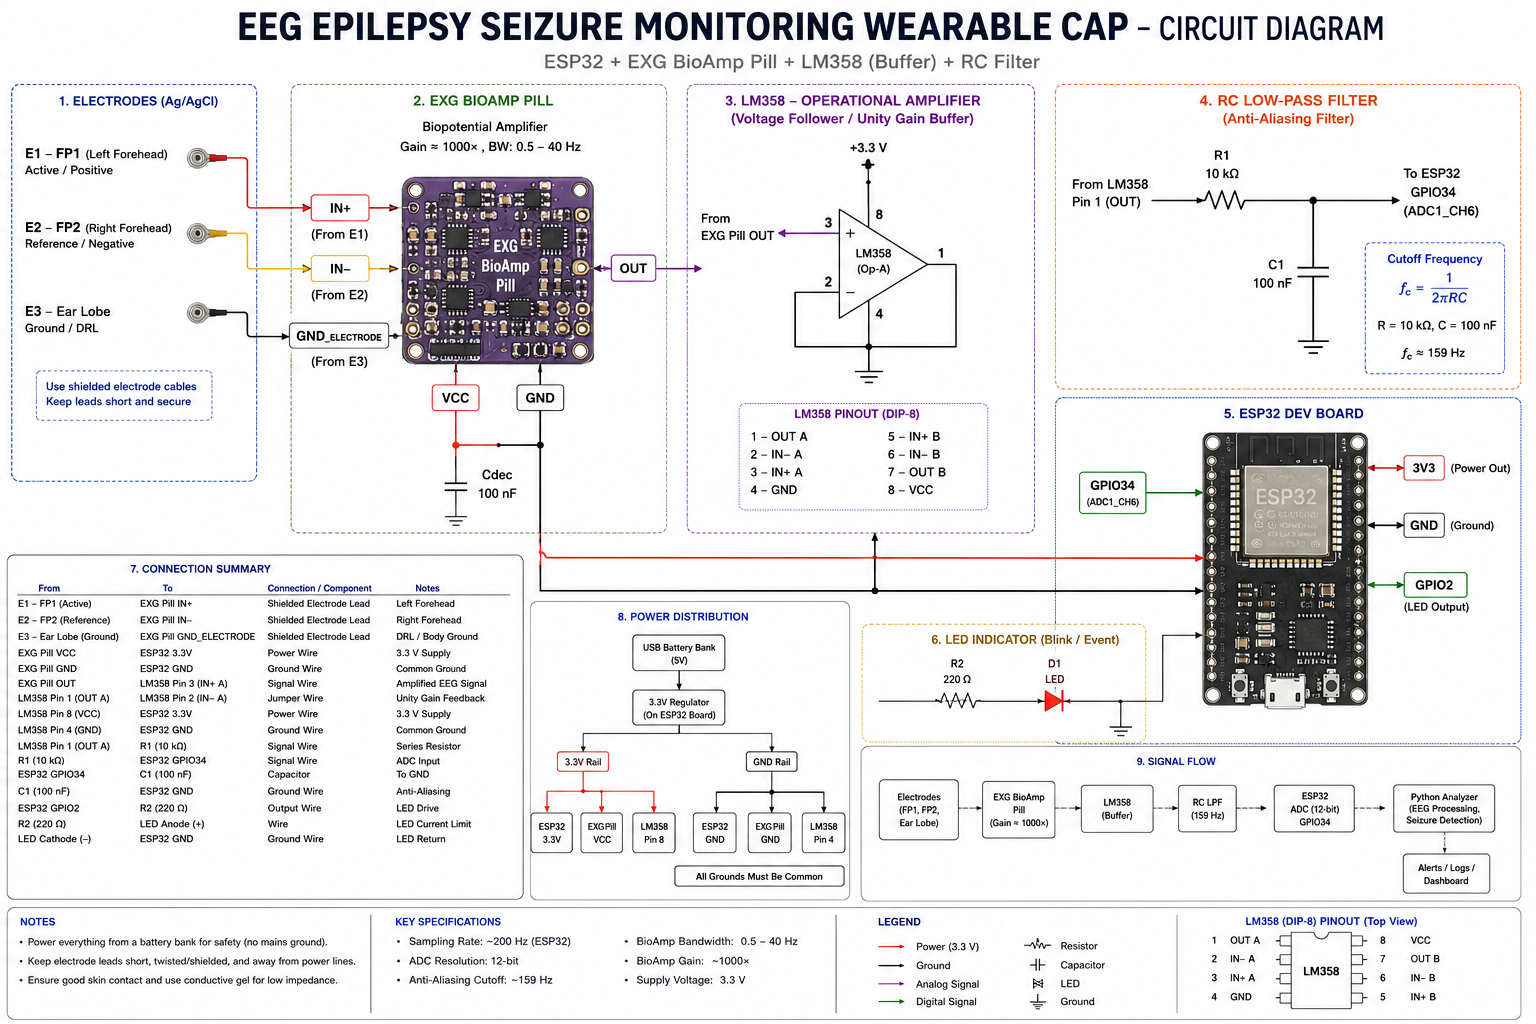
\includegraphics[width=0.84\textwidth]{figures/circuit_diagram.png}
\caption{Prototype schematic from the project documentation: Ag/AgCl electrodes (FP1+, FP2$-$, earlobe ground), EXG BioAmp Pill, LM358 voltage follower, RC low-pass filter and ESP32 (12-bit ADC, GPIO34). Gain and pass-band are the documented nominal values; they have not been measured.}
\label{fig:hw}
\end{figure*}

% =============================================================================
\section{Introduction}
Epilepsy affects about 50 million people~\cite{who2024epilepsy}. Many seizures go unwitnessed, especially at night. Unwitnessed convulsive seizures are a major risk factor for sudden unexpected death in epilepsy~\cite{devinsky2016sudep}, and patient diaries miss a large share of events~\cite{elger2018underreporting}. The ILAE--IFCN guideline endorses wearable detectors only for generalized or focal-to-bilateral tonic--clonic seizures. The devices it endorses sense movement, muscle activity or autonomic signals, and they reached 90--96\% sensitivity with 0.2--0.67 false alarms per day in phase-3 studies~\cite{beniczky2021guideline,onorati2017embrace}. Non-convulsive seizures appear only in the EEG.

Open biopotential front-ends~\cite{frey2016openbci,bioamp} and Wi-Fi microcontrollers~\cite{esp32} make a single-channel EEG alarm cheap to build. Validation is their weak point. Thresholds are tuned by hand, ``pre-ictal'' states are asserted without evidence, and algorithms are usually re-implemented for evaluation rather than tested as the code that ships. We built such a device and then asked two questions. How well does its code, exactly as shipped, detect annotated seizures? And what is the smallest change that makes it useful? The contributions are as follows; the status of each is stated explicitly:
\begin{enumerate}
\item \textbf{A built prototype}: a battery-powered FP1--FP2 EEG monitor with ESP32 firmware, a desktop analyzer and an offline Wi-Fi alert path (Sec.~\ref{sec:system}).
\item \textbf{Code-faithful replay}: the unmodified analyzer and a line-by-line firmware port are run on public EEG converted exactly to the device montage, under a simulated clock. Scoring is event-based, with subject-level validation and an empirical null (Sec.~\ref{sec:method}).
\item \textbf{A diagnosis} of why the shipped detectors fail, at the level of features and design choices (Sec.~\ref{sec:diag}).
\item \textbf{DEV-BR}: a delayed-median ratio rule on the firmware's existing deviation signal, robust in simulation to gain, clipping, ADC-range and sampling-rate deviations, and implemented in 2.5~KB of verified C++ (not yet deployed). Richer rules and learned classifiers did not beat it (Sec.~\ref{sec:devbr}).
\end{enumerate}

% =============================================================================
\section{Related Work}
Scalp-EEG seizure detection dates to Gotman's 1982 detector~\cite{gotman1982}; Baumgartner and Koren review the field~\cite{baumgartner2018scalp}. Line-length is a cheap and effective onset feature~\cite{esteller2001linelength}. Normalizing it against a running memory of past EEG, including median- and window-based memories, measurably changes detection performance~\cite{logesparan2011norm,logesparan2015norm}. Baseline normalization is therefore not new. What we add is to apply it to a signal an existing low-cost firmware already computes, with a lag and persistence rule, under embedded constraints, and to evaluate it against that firmware's own code. On CHB-MIT, patient-specific classifiers that use all 23 channels detect most seizures within seconds~\cite{shoeb2010icml}. Reduced montages such as behind-the-ear EEG retain useful but lower sensitivity~\cite{gu2018behindear}. Event-based scoring with onset and offset tolerances, and false alarms normalized per hour or per day, are now the recommended practice~\cite{ziyabari2017metrics,dan2025szcore}.

% =============================================================================
\section{The Monitoring System}\label{sec:system}


\begin{table}[t]
\centering
\caption{Implementation status and source of each specification.}
\label{tab:status}
\footnotesize
\setlength{\tabcolsep}{2.5pt}
\begin{tabular}{>{\raggedright\arraybackslash}p{0.2\columnwidth}>{\raggedright\arraybackslash}p{0.4\columnwidth}>{\raggedright\arraybackslash}p{0.33\columnwidth}}
\toprule
Item & Specification & Status / source \\
\midrule
Electrodes & Ag/AgCl, FP1$+$/FP2$-$, earlobe ground & built; schematic \\
Amplifier & BioAmp Pill, gain $\approx$1000, 0.5--40~Hz, 3.3-V supply & built; nominal, not measured; vendor documents 5-V use~\cite{bioamp} \\
Buffer, filter & LM358 follower; RC 10~k$\Omega$/100~nF ($f_c{\approx}$159~Hz) & built; schematic \\
ADC, sampling & 12-bit, default attenuation; \texttt{delay(5)}-paced loop ($\approx$200~Hz) & firmware; rate not measured \\
Alarm outputs & RGB LED, 500-ms GPIO pulse, REST \texttt{/status} & firmware \\
Network & ESP32 access point; \texttt{/status}, \texttt{/eeg}, \texttt{/simulate} & firmware \\
Detectors & firmware state machine; 3-feature analyzer & code; replay-evaluated \\
Companion app & Android client of the REST API & binary only; not evaluated \\
DEV-BR & C++ header, 2.5~KB RAM & verified offline; robustness simulated; not deployed \\
Bench data & noise, battery life, cost & not measured \\
\bottomrule
\end{tabular}
\end{table}

\textbf{Hardware.} One differential forehead channel (Fig.~\ref{fig:hw}) is amplified by the BioAmp Pill~\cite{bioamp}, buffered by an LM358 and digitized by the ESP32 (Table~\ref{tab:status}). Forehead sites are hair-free, which suits gel-free consumer use, but they also pick up ocular and muscle artifacts. The device has no galvanic isolation and runs only from a USB battery bank. Two design limits follow from the datasheets rather than from measurement. First, the LM358 is not rail-to-rail: its input common-mode range and output swing end about 1.5~V below the supply~\cite{lm358}, which at 3.3~V leaves roughly 150~mV of positive headroom above the mid-supply output. Second, the firmware leaves the ESP32 ADC at its default attenuation and paces sampling with \texttt{delay(5)}, so the true rate is below the nominal 200~Hz and jitters. Neither effect has been measured on the prototype.

\textbf{Firmware detector (shipped).} For each sample $x[n]$, the firmware tracks a baseline $b[n]{=}0.99\,b[n{-}1]{+}0.01\,x[n]$ (time constant $\approx$0.5~s) and a deviation $d[n]{=}|x[n]-\lfloor b[n]\rfloor|$. In the NORMAL state, $d$ updates an exponentially weighted mean $\mu$ and spread $\sigma$ (forgetting factor 0.995 per sample). After a 90-s warm-up, the BROWNOUT and BLACKOUT thresholds are reset every 30~s to $\mu{+}2.5\sigma$ and $\mu{+}4\sigma$, clamped to [60,\,1200] and [120,\,2400] ADC units. Leaky counters require 20 (BROWNOUT) or 15 (BLACKOUT) samples above threshold, and BLACKOUT ends in a 400-sample post-ictal hold. State, battery level and a 128-sample waveform are served over REST, and the phone app polls them.

\textbf{Desktop analyzer (shipped).} A Python analyzer reads the serial stream. Every 20 samples it computes line-length (LL), the delta/alpha power ratio (DAR) and the 30--45-Hz energy ratio (HFE) over 512 samples (2.56~s). Each feature has adaptive thresholds at $\mu{+}2.5\sigma$ and $\mu{+}4\sigma$ with fixed floors (LL: 300 and 600 units). A state requires two of the three features to agree on 7 of 8 consecutive ticks. Epochs with LL above 1500 are rejected as artifacts, and adaptation freezes during BLACKOUT.

% =============================================================================
\section{Code-Faithful Replay}\label{sec:method}
\textbf{Data and montage.} We used the CHB-MIT Scalp EEG Database~\cite{shoeb2009thesis,goldberger2000physionet}: 256~Hz, 16-bit, 24 cases from mostly pediatric subjects aged 1.5--22 years. Case chb21 is the subject of chb01 recorded 1.5 years later, and no subject information is given for chb24, which we treat as a separate subject. We took all 141 recordings that contain seizures plus one seizure-free recording per case (two for chb01; none listed for chb24), \NRecAll{} recordings in all (\NSzAll{} seizures, \NHoursAll{}~h). The FP1--FP2 derivation is not stored directly. We reconstructed it exactly as the signed sum of the bipolar chain FP1-F7, F7-T7, T7-FT9, FT9-FT10, FT10-T8, $-$(F8-T8), $-$(FP2-F8), or as FP1$-$FP2 for the few referential files. Five recordings lack this chain (chb13\_40, chb16\_18, chb15\_01, chb18\_01, chb19\_01). The two with seizures hold 4 seizures, which leaves \NRec{} recordings, \NSz{} seizures and \NHours{}~h on FP1--FP2, the primary channel. FP1-F7 and FP2-F8 serve as secondary channels.

\textbf{Front-end model.} Each channel passes through a causal model of the nominal analog pass-band: a first-order 0.5-Hz high-pass and a second-order 40-Hz Butterworth low-pass. It is then resampled to 200~Hz with a polyphase filter, offset to 1.65~V, scaled by the nominal gain of 1000 and quantized to 12~bits over 3.3~V. This model does not include electrode impedance, motion, mains interference, LM358 headroom or ESP32 ADC nonlinearity.

\textbf{Running the shipped code.} The analyzer (\texttt{seizure\_monitor.py}) is imported unmodified. Its own serial-reader loop is driven by a simulated serial port that emits the firmware's output format, and by a simulated clock that advances 5~ms per sample, so warm-up, re-adaptation and confirmation behave exactly as the code specifies. Only plotting, logging and network alerts are stubbed. The firmware's \texttt{loop()} is ported line by line, including integer casts and the 200-sample boot calibration, and JIT-compiled. Its output forms the analyzer's input stream. Every recording starts from a fresh device state. This is a software replay: no hardware-in-the-loop experiment was performed.

\textbf{Scoring and statistics.} Following SzCORE~\cite{dan2025szcore}, an alarm is an entry into an alarm state. Alarms less than 90~s after the previous one are merged. A seizure counts as detected if an alarm falls within [onset$-$30~s, offset$+$60~s]; every other alarm is a false alarm (FA). FA/h uses total recording time, which differs from inter-ictal time by under 2\%. We report pooled sensitivity and the subject-macro average. 95\% CIs come from a 2000-resample subject-level bootstrap. Detectors are compared per subject with the Wilcoxon signed-rank test (23 subjects). As an empirical null, each detector's alarm train is circularly shifted by a random offset within every recording, which preserves alarm count and spacing, and rescored \NPerm{} times.

% =============================================================================
\section{Why the Shipped Detectors Fail}\label{sec:diag}
\begin{table*}[t]
\centering
\caption{Event-based results on FP1--FP2 (\NSubj{} subjects, \NSz{} seizures, \NHours{}~h; nominal front-end). Brackets: subject-bootstrap 95\% CI. ``Macro'': mean of per-subject sensitivities. ``Chance'': mean sensitivity of the same alarm train circularly shifted at random. Baseline-ratio (BR) detectors: held-out subjects only (leave-one-subject-out).}
\label{tab:main}
\begin{tabular}{lcccccc}
\toprule
Detector & Detected & Sensitivity [95\% CI] & Macro & FA/h & Latency (s) & Chance \\
\midrule
\MainTableBody
\bottomrule
\end{tabular}
\end{table*}

\textbf{Outcomes.} The analyzer's BLACKOUT alarm detected \PyBDet{}/\NSz{} seizures (\PyBSens{}) at \PyBFAh{}~FA/h (Table~\ref{tab:main}). Counting BROWNOUT warnings as alarms raised sensitivity to \PyASens{} but also raised false alarms to \PyAFAh{}~FA/h. The firmware detector reached \FwBSens{} at \FwBFAh{}~FA/h (about \FwBFAday{} per day), but its circularly shifted alarms already reach \FwBNull{}. Its spread estimate has a memory of about 1~s (forgetting factor 0.995 at 200~Hz), so a 4$\sigma$ excursion lasting 75~ms is routine in ordinary EEG. All three shipped outputs exceed their nulls ($p\le\ShipNullMaxP$), so they carry some seizure information, but too little at a usable alarm rate.

\begin{figure*}[t]
\centering
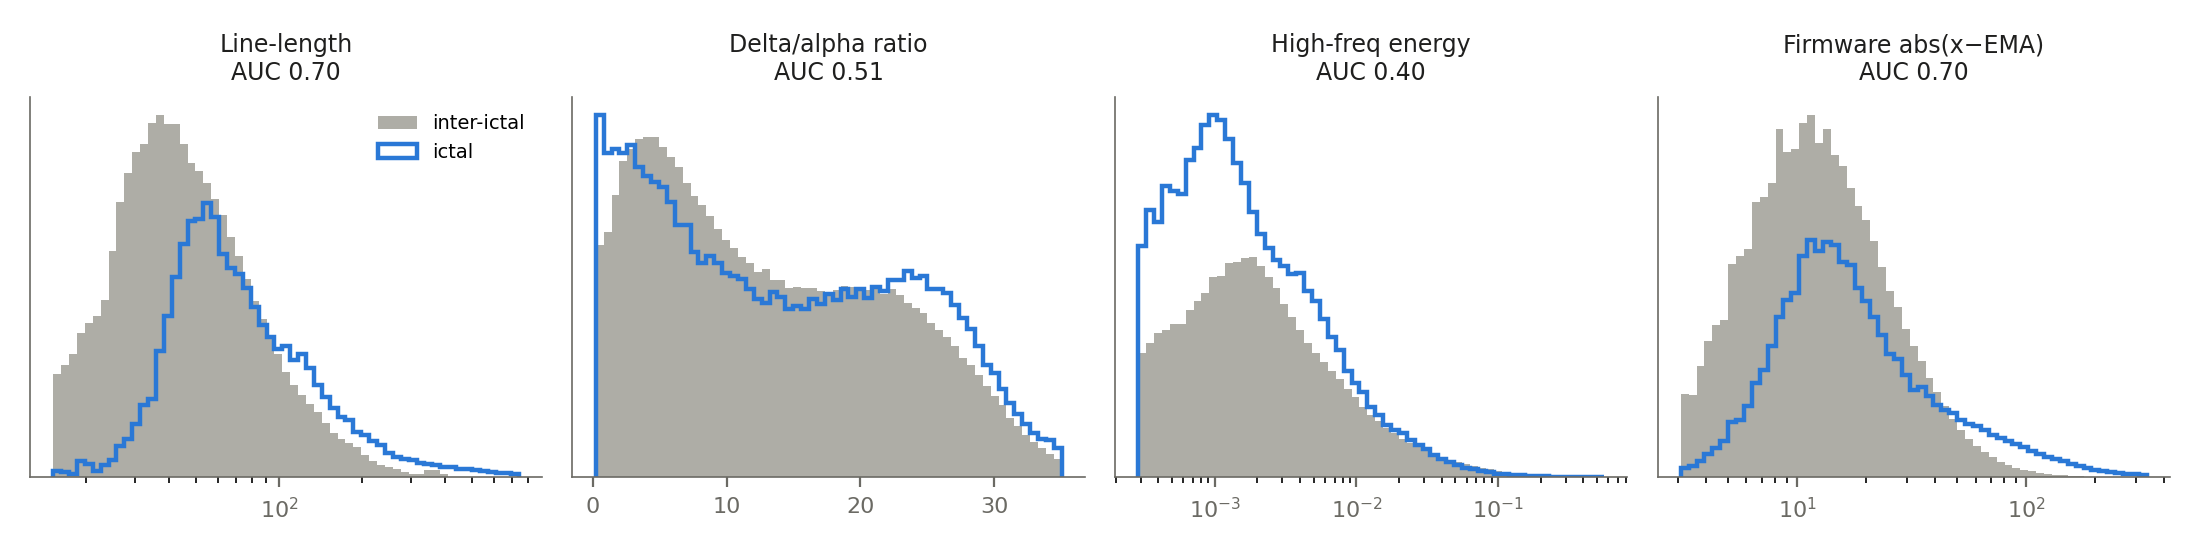
\includegraphics[width=0.92\textwidth]{figures/feature_distributions.png}
\caption{Ictal (blue) versus inter-ictal (grey) distributions on FP1--FP2 of the analyzer's three features and the firmware deviation $d$ (100-ms means), with the pooled AUC.}
\label{fig:feat}
\end{figure*}

\textbf{Feature evidence.} Line-length (pooled AUC \AucLL{}; median per subject \AucLLCase{}) and the firmware deviation (AUC \AucFW{}; per subject \AucFWCase{}) separate ictal from inter-ictal ticks (Fig.~\ref{fig:feat}). DAR is at chance (\AucDAR{}). HFE is below chance (\AucHFE{}), so ictal ticks carry \emph{less} 30--45-Hz energy than inter-ictal ones. A plausible but untested explanation is that this band, near the front-end's 40-Hz roll-off, is dominated by forehead muscle activity. The 2-of-3 vote therefore needs agreement from features that carry no seizure information. Two further problems follow from the design. The fixed LL floors are absolute ADC values, so detection depends on amplifier gain: at gains of 500, 1000 and 2000 the BLACKOUT sensitivity was \PyBSensLowGain{}, \PyBSens{} and \PyBSensHighGain{}. And per-subject AUCs exceed the pooled ones, so background levels differ between people and no fixed threshold suits everyone.

% =============================================================================
\section{DEV-BR: A Delayed-Median Ratio Detector}\label{sec:devbr}
The diagnosis suggests normalizing against each wearer's own slowly varying background rather than a 1-s window, requiring persistence on the order of seconds, and avoiding absolute units. DEV-BR applies these to the deviation $d$ the firmware already computes. With $t$ indexing whole seconds:
\begin{align}
\delta(t) &= \mathrm{mean}\{\,d[n] : n \text{ in second } t\,\},\\
\beta(t) &= \mathrm{median}\{\,\delta(\tau) : t{-}329 \le \tau \le t{-}30\,\},\\
\text{alarm at } t{+}1 &\iff \delta(\tau) \ge r\,\beta(\tau)\;\; \forall\,\tau \in [t{-}D{+}1,\, t]
\end{align}
The alarm fires on the first second the condition holds, and alarms within 90~s of the previous one are suppressed. No alarm is possible before $t{=}330$~s. The 30-s lag keeps a seizure's onset out of its own baseline. LL-BR applies the same rule to line-length, and FUSE-BR to the geometric mean of the two ratios. Multiplying the signal by a constant leaves $\delta/\beta$ unchanged except through quantization and saturation, so the rule is invariant to amplifier gain only in that sense.

\textbf{Parameter selection.} The threshold $r\in\{1.25,\dots,8\}$ and persistence $D\in\{2,\dots,30\}$~s are chosen by leave-one-subject-out cross-validation (LOSO, 23 folds). On the 22 training subjects we pick the most sensitive $(r,D)$ whose FA/h meets a target, then apply it to the held-out subject. To avoid choosing the signal after seeing the results, a nested variant also selects the signal (LL, DEV or FUSE) inside each training fold. It selected DEV in \NestedDev{} of \NestedAll{} folds, so its results equal those of DEV-BR. The baseline window (300~s) and lag (30~s) were fixed after a 9-recording pilot drawn from the same database, before the full evaluation, and are examined by ablation below.

\textbf{Embedded implementation.} A header-only C++ class implements DEV-BR with a 330-value history ring and a 300-value scratch array. It computes the median with \texttt{std::nth\_element} once per second and needs about 2.5~KB of RAM. Fed the evaluation's per-second deviation series for all \NRec{} recordings at five parameter settings, it reproduced every alarm time of the Python evaluation (800 of 800 runs identical). It has not yet been integrated into the firmware or timed on the ESP32.

\begin{figure}[t]
\centering
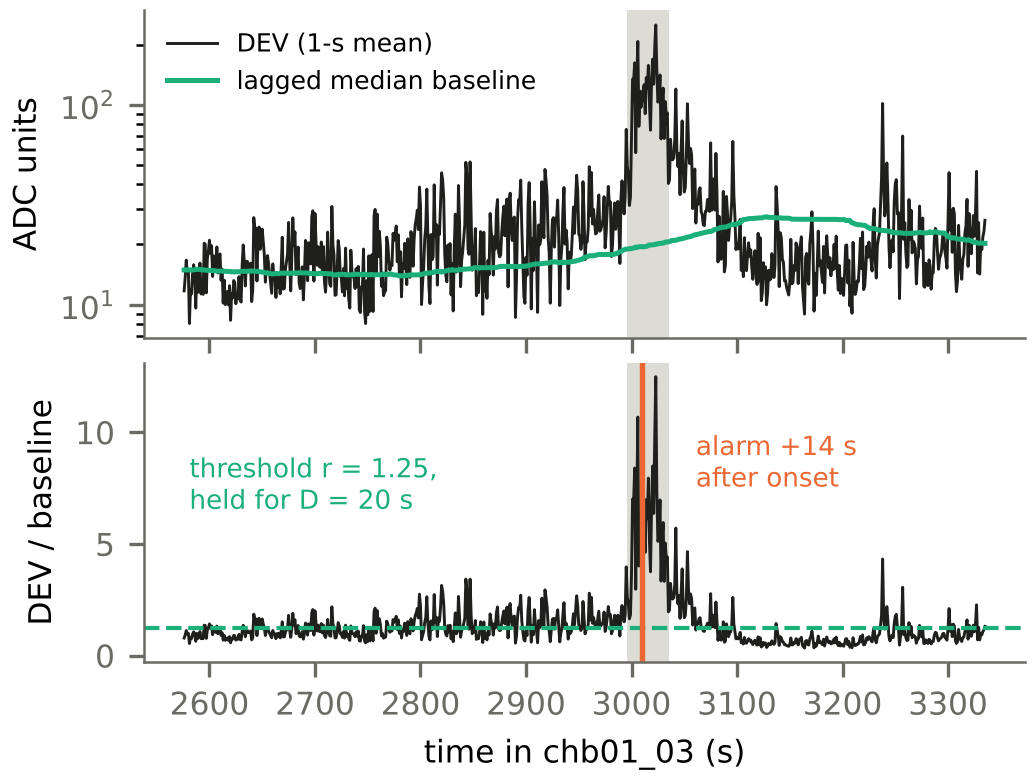
\includegraphics[width=0.9\columnwidth]{figures/devbr_example.png}
\caption{DEV-BR on a seizure in chb01 (shaded). Top: the per-second deviation and its delayed median baseline. Bottom: their ratio, the modal held-out threshold, and the alarm.}
\label{fig:example}
\end{figure}

\begin{figure}[t]
\centering
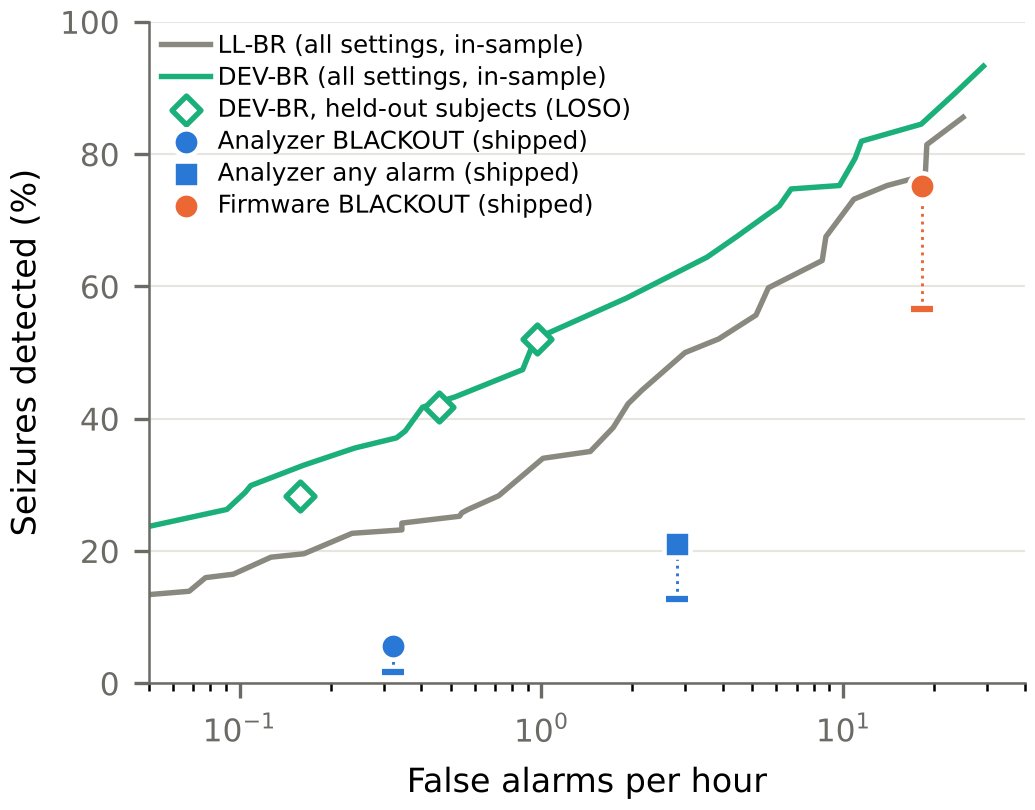
\includegraphics[width=0.88\columnwidth]{figures/operating_curve.png}
\caption{Sensitivity versus FA/h on FP1--FP2. Lines: the best trade-off over all ratio settings, in-sample. Diamonds: DEV-BR on held-out subjects. Markers: the shipped detectors, with dashes at their circular-shift chance levels.}
\label{fig:roc}
\end{figure}

\textbf{Results.} On held-out subjects, DEV-BR detected \DevADet{}/\NSz{} seizures (\DevASens{}, CI \DevACI{}; subject-macro \DevAMacro{}) at \DevAFAh{}~FA/h, with a median latency of \DevALat{}~s (Table~\ref{tab:main}, Figs.~\ref{fig:example}--\ref{fig:roc}). The most frequent choice across folds was $r{=}\DevAR$, $D{=}\DevAD$~s (\DevAModeCount{} of \DevAFolds{} folds). Stricter targets gave \DevBSens{} at \DevBFAh{}~FA/h and \DevCSens{} at \DevCFAh{}~FA/h. At a false-alarm rate comparable to the analyzer's BLACKOUT alarm, DEV-BR detected about \FoldDevPy{} times as many seizures. It did better in \TestDevPyBetter{} of \TestDevPyN{} subjects, worse in \TestDevPyWorse{} and tied in \TestDevPyTies{} (\TestDevPyP{}). It also outperformed LL-BR (\TestDevLlBetter{} better, \TestDevLlWorse{} worse, \TestDevLlP{}). Its circular-shift chance level was \DevANull{} (\DevANullP{}). The original 2-fold split gave \TwoDevASens{} at \TwoDevAFAh{}~FA/h. Excluding the \NColdStart{} seizures that start before the 330-s warm-up raises sensitivity to \DevASensWarm{}. On the secondary channels, DEV-BR detected \DevSensOne{} (FP1-F7) and \DevSensTwo{} (FP2-F8) at $\le$1~FA/h, but its advantage over LL-BR there was not significant (\SecLlPOne{}, \SecLlPTwo{}; Table~\ref{tab:abl}).

\begin{table}[t]
\centering
\caption{Top: DEV-BR ablations and alternative detectors (all LOSO, FP1--FP2; learned models use inner cross-validation for thresholds), sensitivity / FA/h at the $\le$1 and $\le$0.5~FA/h targets. Bottom: secondary channels at $\le$1~FA/h.}
\label{tab:abl}
\footnotesize
\setlength{\tabcolsep}{3pt}
\begin{tabular}{lcc}
\toprule
Variant & $\le$1 FA/h & $\le$0.5 FA/h \\
\midrule
\AblationTableBody
\bottomrule
\end{tabular}

\vspace{3pt}
\setlength{\tabcolsep}{2pt}
\begin{tabular}{lcccc}
\toprule
Channel & Analyzer (any) & Firmware & LL-BR & DEV-BR \\
\midrule
\SecondaryTableBody
\bottomrule
\end{tabular}
\end{table}

\textbf{Ablations.} Normalization is the essential ingredient: thresholding the raw deviation, with the threshold also chosen by LOSO, detected only \AblAbsSens{} at a similar FA/h (Table~\ref{tab:abl}). Removing the lag cost sensitivity at the stricter target (\AblLagZeroSensB{}), and a 600-s window performed worse than 60--300~s. A mean baseline performed about as well as the median (\AblMeanSens{}), so the median offers robustness to outliers rather than a performance gain.

\textbf{Is a more complex detector better?} We tested k-of-n persistence, a dual time-scale rule, a baseline carried across contiguous recordings, and learned classifiers on 14 baseline-normalized features: logistic regression (an embedded-friendly dot product) and gradient-boosted trees. Their thresholds were chosen by inner cross-validation within each training fold. None consistently beat DEV-BR (Table~\ref{tab:abl}). Boosted trees were better at the stricter target (\GbmHalfSens{} versus \DevBSens{}; \GbmHalfBetter{} subjects better, \GbmHalfWorse{} worse, \GbmHalfP{}) and worse at $\le$1~FA/h, at a far higher computational cost. On one forehead channel, the simplest rule already sits at the information limit of the signal, so further gains must come from sensing, such as a second electrode, rather than from the algorithm.

\ifnum\HwAvailable=1
\begin{table}[t]
\centering
\caption{Front-end robustness of DEV-BR (FP1--FP2, simulated). ``Fixed'': parameters chosen at gain 1000 ($r{=}\HwFixR$, $D{=}\HwFixD$~s) applied unchanged. LM358 clip: 1.8-V output ceiling; Sat.: saturated samples. Cells: sensitivity / FA/h.}
\label{tab:hw}
\footnotesize
\setlength{\tabcolsep}{1.5pt}
\begin{tabular}{lcccc}
\toprule
Condition & Sat. & DEV-BR fixed & DEV-BR LOSO & Firmware \\
\midrule
\HwTableBody
\bottomrule
\end{tabular}
\end{table}
\textbf{Front-end robustness.} Table~\ref{tab:hw} reruns the firmware stage under different gains, the LM358 output ceiling, the ESP32's default ADC range and a 6-ms loop, with DEV-BR's parameters frozen at gain 1000. DEV-BR's sensitivity stayed within \HwDevSensMin{}--\HwDevSensMax{} at \HwDevFAMin{}--\HwDevFAMax{}~FA/h, and it was identical (\HwGainSens{}) at gains of 500, 1000 and 2000. Even at gain 2000 with the LM358 ceiling, where \HwClipSat{} of samples saturated, it detected \HwClipSens{}. The shipped firmware's operating point moved between \HwFwSensMin{} and \HwFwSensMax{} sensitivity and \HwFwFAMin{}--\HwFwFAMax{}~FA/h.
\else
\textbf{Front-end robustness.} The scale argument above has not yet been confirmed by rerunning DEV-BR at gains of 500 and 2000, under the LM358 output ceiling, or at a slower sampling rate. The released add-on notebook performs these runs. For the shipped detectors, firmware false alarms changed from \FwBFAhLowGain{} to \FwBFAhHighGain{}~FA/h between gains of 500 and 2000.
\fi



% =============================================================================
\section{Discussion and Limitations}
Code-faithful replay changed how the prototype's alarms should be described, and it showed how to fix them. The shipped on-device detector mostly fires at random, and the analyzer's ``pre-ictal'' BROWNOUT state has no demonstrated predictive value. A different decision rule on a signal the firmware already computes turns the alarm into a significant, hardware-robust detector at about one false alarm per hour, with no new sensing or hardware cost. Three principles generalize to other low-cost biosignal devices: validate the code that ships rather than a re-implementation; normalize against the wearer's own delayed background so that decisions are invariant to gain and front-end tolerances; and stop adding algorithmic complexity once held-out tests show the signal is the bottleneck.

The absolute numbers matter as much as the relative gain. About half of seizures at roughly one false alarm per hour (about 23 per day) is far from the 0.2--0.67 false alarms per day of wearables validated in phase-3 studies for tonic--clonic seizures~\cite{beniczky2021guideline}. It is also below multichannel patient-specific detectors~\cite{shoeb2010icml}. The device is a research prototype, not a medical device, and these results support no clinical claim.

The study has several limitations. (i)~All results come from software replay of a pediatric dataset recorded with clinical amplifiers; no recordings from the prototype are reported. (ii)~The front-end model uses nominal, unmeasured gain and pass-band values. LM358 clipping, ADC range and sampling rate were tested only in simulation, and ADC nonlinearity, timing jitter, electrode impedance, motion and mains interference are not modelled. (iii)~The BioAmp is powered at 3.3~V, below its documented 5-V use. (iv)~Each recording starts cold, which penalizes the \NColdStart{} seizures that begin in the first 330~s; continuous wear would not have this problem. (v)~A forehead channel cannot see every seizure. (vi)~CHB-MIT subjects contribute unequal numbers of seizures (chb12: 40), hence the macro averages. (vii)~DEV-BR runs offline only, and the access point uses a fixed password. The next steps, in order, are bench characterization (noise, gain, sampling rate, battery life), deploying DEV-BR on the device, replacing the LM358 with a rail-to-rail buffer, and a supervised recording study under ethics approval.

% =============================================================================
\section{Conclusion}
We built a low-cost single-channel EEG seizure alarm and evaluated its shipped detection code as written, by replaying \NSubj{} subjects of annotated EEG through a model of its front-end. The shipped detectors fail for identifiable reasons: short-memory adaptation, gain-dependent thresholds and a vote dominated by uninformative features. A firmware-only upgrade, DEV-BR, fixes these. It detected \DevASens{} of seizures at \DevAFAh{}~FA/h on held-out subjects, about \FoldDevPy{} times the shipped analyzer at a comparable false-alarm rate. It kept that performance essentially unchanged across a fourfold range of amplifier gain and under clipping, ADC-range and timing deviations, and it fits in 2.5~KB of RAM. More complex detectors did not improve on it, so the next gains will come from additional sensing, which together with clinical-grade false-alarm rates remains future work. Hardware, firmware, analyzer, replay benchmark and the C++ detector are released for others to reproduce and extend.

\section*{Data and Code Availability}
CHB-MIT is available from PhysioNet~\cite{goldberger2000physionet}. Firmware, analyzer, schematics, the replay benchmark (with Kaggle notebooks) and the DEV-BR C++ header are at~\cite{vera_repo}. The companion app is distributed there as a binary.

\section*{Acknowledgment}
The authors used an AI assistant (Claude, Anthropic) to help develop the evaluation code and draft the manuscript; the authors reviewed all content and take full responsibility for it.

\bibliographystyle{IEEEtran}
\bibliography{refs}

\end{document}
